\documentclass[twocolumn]{revtex4-2}
\usepackage{amsmath}
\usepackage{graphicx}% Include figure files
\usepackage{dcolumn}% Align table columns on decimal point
\usepackage{xcolor}
\usepackage[section]{placeins}

\usepackage[hyperfootnotes=true]{hyperref}
\hypersetup{colorlinks, citecolor=blue, linkcolor=red, urlcolor=purple}


\begin{document}

\preprint{APS/123-QED}

\title{Self-similar Worthington jets} % Force line breaks with \\

\author{Jos\'e M. Gordillo$^{1}$}
\email{jgordill@us.es}
\author{Javier Rodr\'iguez--Rodr\'{i}guez$^{2}$}%
\author{Vatsal Sanjay$^{3}$}
\affiliation{$^1$\'Area de Mec\'anica de Fluidos, Departamento de Ingenier\'ia Aeroespacial y Mec\'anica de Fluidos, Universidad de Sevilla, Avenida de los Descubrimientos s/n 41092, Sevilla, Spain
}
\affiliation{$^2$ Department of Thermal and Fluids Engineering,
“Gregorio Millán Barbany” Institute, Universidad Carlos III de Madrid, Spain}
\affiliation{$^3$CoMPhy Lab, Department of Physics, Durham University, Science Laboratories, South Road, Durham
DH1 3LE, United Kingdom}

\date{\today}% It is always \today, today,

\begin{abstract}
When a micron-sized bubble bursts, capillary waves deform the cavity into a cone that ejects a Worthington jet. The jet is born by inertial focusing, and the local collapse follows self-similar Euler solutions set by the semiangle $\beta$. Writing $r_j$ and $v_j$ for the dimensionless jet-base radius and velocity, the local Weber number $We_j=r_j v^2_j$ measures inertia relative to capillarity. The theory, supported by accurate numerical simulations gives $r_j\propto\tau^{\alpha(\beta)}$ with $\alpha\simeq0.63$ and, hence $We_j\gg1$, with $We_j\to\infty$ as $r_j\to0$, so inertia increasingly overwhelms capillarity. In simulations, the interface collapses onto a universal shape for more than two decades in dimensionless time when lengths are scaled using our prediction for $r_j$. For water, this gives incipient radii of $\mathcal{O}(1)$ nm, predicting nanometric sea-spray aerosols.
\end{abstract}

\maketitle

Bubble bursting ejects Worthington jets whose breakup transfers material across liquid--gas interfaces, from sea spray \cite{MacIntyre,Bigg,PNAS,AnnRevDeike,JFMGanan,Gananfinespray,PNASWang,Abyss} and rain-induced aerosols \cite{RainPorous} to sparkling wines \cite{SeonLigerBelair2017} and electrochemical sprays \cite{Bashkatov2025}. The jet dynamics and minimum drop sizes are set by capillary-wave focusing \cite{Duchemin,Walls2015,krishnan2017,PRFBird,Deike,Berny}. The radii $R$ of the bubbles for which submicrometric droplets can be produced via bubble bursting jets in a surfactant-free or negligibly contaminated interface of a liquid of density $\rho$, dynamic viscosity $\mu$ and interfacial tension coefficient $\sigma$, is characterized by a value of the Ohnesorge number $Oh=\mu/\sqrt{\rho R\sigma}\approx0.03$ \cite{Walls2015,PRFBird}; for water, this means micron-sized bubbles with $Bo=\rho gR^2/\sigma\ll1$, with $g$ indicating gravity \footnote{In the following, lower-case letters indicate dimensionless variables defined using $R$, the capillary velocity $V_c=\sqrt{\sigma/(\rho R)}$, and $\rho V_c^2$ as the characteristic values of length, velocity and pressure. In the limit $Bo\rightarrow0$, the pre-inception bubble-bursting dynamics are controlled by $Oh$, or equivalently $La=Oh^{-2}$; gas properties become relevant after ejection through the drag exerted on the jet tip and emitted droplets \cite{JFM2020,Tian2023}.}. In this regime, capillary waves deform the bubble into a conical cavity of semiangle $\beta$ and entrap a tiny bubble beneath the cavity before the fastest, thinnest jet is emitted \cite{JFM2019,JFM2020} (Figs.~\ref{fig:sketch_problem} and~\ref{fig:data-figs}(a)(i)--(iv)). The local question is what similarity law governs the focusing flow after this conical cavity has formed. Far from being an academic problem, a precise description of the physical laws that govern the jet's formation is essential to accurately predict the size of the resulting ejected drop which, eventually, will turn into the aerosol particle.

In the classical inertio-capillary interpretation, dynamic and capillary pressures balance during collapse, giving $r_j\propto\tau^{2/3}$ and a local Weber number $We_j=v_j^2r_j=\mathcal{O}(1)$ \cite{Zeff,Duchemin,Sierou,PRLEggers,PRLCattaneo}. This interpretation is difficult to reject from the exponent alone, because bubble-bursting simulations give values close to $2/3$ and previous rescalings with $\tau^{2/3}$ do collapse the evolving interface over a limited time interval \cite{Zeff,PRLEggers,PRLCattaneo}. However, the exponent alone is a weak balance test. The local Weber number gives a more direct test of the balance, since the inertio-capillary picture requires $We_j$ to remain order unity and independent of $r_j$. Our direct numerical simulations instead show that the jet-base Weber number is large, $We_j\gg1$, and grows toward the singular $r_j \to 0$ limit (Fig.~\ref{fig:data-figs}(c)).
\begin{figure}
    \centering
    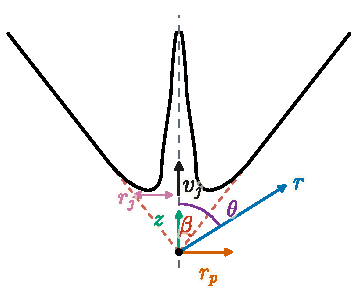
\includegraphics[width=0.8\linewidth]{sketch_paper_worthington.pdf}
    \caption{Schematic of the inertial conical-collapse problem. The gas cavity approaches a cone of semiangle $\beta$, described using the polar distance $r$ and angle $\theta$ measured from the apparent apex, or equivalently the axial and radial coordinates $z$ and $r_p$. The jet radius $r_j$ and velocity $v_j$ define the local observables used to test the self-similar scaling.}
    \label{fig:sketch_problem}
\end{figure}

Here we solve the corresponding conical-collapse problem as a local inertial-focusing problem. Capillarity and viscosity, through $Oh$, select whether the system enters the singular regime --when the tiny bubble is entrapped and the ejected jet is the fastest--, and set the cone angle $\beta(Oh)$ and jet inception time. Once the similarity window $r_j\ll r\ll1$ exists with $r$ the polar distance, see Fig.~\ref{fig:sketch_problem}, the dominant balance must be inertial owing to the very large values of the local Weber number. The exponent in $r_j\propto \tau^{\alpha(\beta)}$ is therefore not universal but fixed by the far-field cone geometry through $\alpha(\beta)=1/(2-\nu(\beta))$, with $\nu(\beta)$ fixed by the condition $P_\nu(-\cos\beta)=0$, where $P_\nu$ indicates the Legendre function of degree $\nu$. Dependence on the initial or far-field cavity geometry, also observed in recent cavitation and shallow-layer bubble-bursting jets \cite{PRL2024,YangShallow2026}, is a signature of a second-kind similarity rather than a secondary correction. In shallow-layer bursting, for example, wall proximity steepens the focusing cavity and reduces the emitted drop size \cite{YangShallow2026}, consistent with a geometry-induced change in $\beta$.

We derive this family of Euler self-similar solutions, test it against direct numerical simulations at $Oh=0.03$, and show that the same solution collapses the interface for more than two decades in dimensionless time. The measured growth of $We_j$ as $r_j \to 0$ tests the force balance, and the trend $\alpha[\beta(Oh)]<2/3$ tests the exponent (see End Matter). The resulting viscous cutoff predicts incipient radii of $\mathcal{O}(1)$ nm for water, suggesting a route by which bursting micron-sized bubbles can produce nanometric sea-spray aerosols.


\emph{Conical similarity.}---When the production of vorticity at the interface can be neglected, the velocity field $\mathbf{v}$ can be expressed as the gradient of a velocity potential $\phi$, $\mathbf{v}=\nabla\phi$. In the incompressible limit, $\phi$ verifies the Laplace equation $\nabla^2\phi=0$, which must be solved subject to dynamic and kinematic boundary conditions at the interface $F=r-r_s(\theta,t)=0$, with $\theta$ indicating the polar angle in spherical coordinates centered at the apex of the cone, which is also the origin of distances $r$ (see Fig.~\ref{fig:sketch_problem}). In the limit in which capillary and viscous stresses are negligible, the dynamic boundary condition is the Euler-Bernoulli equation particularized at $F=0$, $\partial\phi/\partial \tau+|\nabla\phi|^2/2=0$, whereas the kinematic boundary condition reads $\partial F/\partial \tau+\nabla\phi\cdot\nabla F=0$.

Since, far away from the jet base, $r\rightarrow\infty$, the interface converges to a cone of semiangle $\theta=\beta$, the problem lacks a spatial scale. Thus, it is natural to seek for a local, self-similar solution. To investigate the structure of the solution, we make use of the scaled variables proposed in Ref. \cite{Zeff},
\begin{equation}
\begin{split}
&\phi=\left(\tau'-\tau_0(Oh)\right)^\delta\,h\left[\frac{z'-\ell_0(Oh)}{\left(\tau'-\tau_0(Oh)\right)^\varepsilon},\frac{r_p}{\left(\tau'-\tau_0(Oh)\right)^\varepsilon}\right] \\ &\mathrm{and}\quad
r_s(z,\tau)=\left(\tau'-\tau_0(Oh)\right)^\varepsilon\,g\left[\frac{z'-\ell_0(Oh)}{\left(\tau'-\tau_0(Oh)\right)^\varepsilon}\right]\, \label{ansatz}
\end{split}
\end{equation}
 with $\tau=\tau'-\tau_0(Oh)$ the dimensionless time and $z=z'-\ell_0(Oh)$, $r_p$ indicating, respectively, the vertical and radial distances in polar coordinates (see Fig.~\ref{fig:sketch_problem}). The system composed of the Laplace equation, the Euler--Bernoulli equation, and the kinematic boundary condition can be written in terms of the variables in Eq. (\ref{ansatz}) if $\delta=2\varepsilon-1$ \cite{Zeff}, with this condition arising from the balance between the temporal and the convective derivatives in the dynamic and kinematic boundary conditions. So far, equation $\delta=2\varepsilon-1$ constitutes the only restriction for self-similar solutions to exist. However, an additional condition that the exponents $\delta$ and $\varepsilon$ must fulfill is deduced by imposing the behavior of the velocity potential $\phi$ in the far field. It has been shown in \cite{PRF2023} that, for the cases $Oh\lesssim 0.02$, i.e., when the bubble bursting jets are issued from the base of a truncated cone, the far-field velocity potential satisfies
\begin{equation}
r_p\frac{\partial\phi}{\partial r_p}\rightarrow -q_\infty\quad\mathrm{for}\quad r_p\rightarrow\infty\, ,\label{qinfty}
\end{equation}
with $q_\infty$ the value of the time-independent far-field flow rate per unit length along the axis of the cone, fixed at the instant when the jet starts to be issued \cite{PRF2023}. Notice that Eqs. (\ref{ansatz}) and (\ref{qinfty}) imply that $\delta=0$ and, hence, $\varepsilon=1/2$ and $r_j(\tau)\propto \tau^{1/2}$, with $We_j\propto \tau^{-1/2}\propto r^{-1}_j$, in agreement with numerical results \cite{PRF2023}.

However, for $0.02\lesssim Oh\lesssim 0.05$ in which jets are issued after a tiny bubble is entrapped at the bottom of the collapsing cavity, the results in Fig.~4(b) of Ref.~\cite{PRF2023} reveal that, right at the instant when the jet begins to be issued, there exists an intermediate spatial region $r_j(\tau)\ll r\ll 1$, also visible qualitatively in the DNS sequence of Fig.~\ref{fig:data-figs}(a)(i)--(iv),
where streamlines are perpendicular to the conical interface \footnote{The spatial region in which streamlines are horizontal in Fig.~4(b) of Ref.~\cite{PRF2023} corresponds to the far-field boundary condition in Eq. (\ref{qinfty}): when the vertical position of the base of the jet reaches this region, $r_j\propto \tau^{1/2}$, $We_j\propto \tau^{-1/2}\propto r^{-1}_j$ for all values of $Oh$, as shown in \cite{PRF2023}.}. Hence, for $0.02\lesssim Oh\lesssim 0.05$, the far field boundary condition driving the ejection of the jet must be a solution of the Laplace equation satisfying the condition $\phi(\theta=\beta)=0$
\footnote{$\phi=0$ is, by virtue of the Euler-Bernoulli equation, the far-field boundary condition for the velocity potential at the interface describing the sudden impact of a solid on an interface \cite{wagner1932} and also describing the type of Worthington jets issued as a consequence of the collapse of slender axisymmetric cavities \cite{PRF2023}.}, which implies that
\begin{equation}
\phi(r\rightarrow\infty)\rightarrow A r^\nu P_\nu(-\cos\theta)=A \tau^{\varepsilon \nu}\left(r/\tau^\varepsilon\right)^\nu P_\nu(-\cos\theta) \label{farfieldBC}
\end{equation}
with the value of the time-independent constant $A$ fixed by the velocity in the far field at the instant when the jet starts to be issued. Equation (\ref{farfieldBC}), together with the far-field condition $\phi(\theta = \beta) = 0$, imposes that the degree of the Legendre function $\nu$ must satisfy the condition
\begin{equation}
P_\nu(-\cos\beta)=0\, .\label{condition}
\end{equation}

\begin{figure*}[t]
\centering
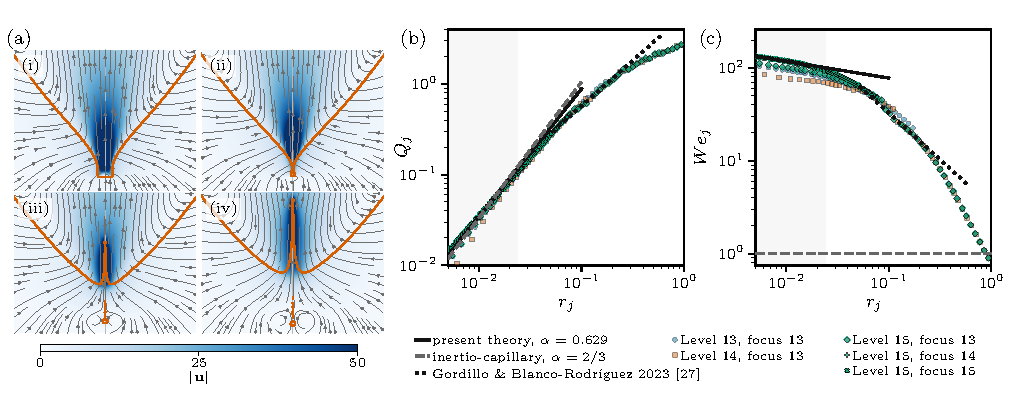
\includegraphics[width=0.95\textwidth]{fig2_v2.pdf}
\caption{DNS evidence for inertial focusing at $Bo=0$ and $Oh=0.03$. (a) Velocity magnitude, streamlines, and interface shapes near jet inception; the four snapshots (i)--(iv) correspond to $\tau-\tau_0=-1.9\times10^{-3}$, $-2.1\times10^{-4}$, $+2.3\times10^{-3}$, and $+5.4\times10^{-3}$, respectively. Orange curves mark the interface, grey curves the streamlines, and colour gives $|\mathbf{u}|$. (b) Jet-feeding flux $Q_j=2\pi\int v_z r\,\mathrm{d}r=\pi r_jq_j$. (c) Local Weber number $We_j=Q_j^2/(\pi^2r_j^3)=q_j^2/r_j$. Symbols show DNS for \texttt{MAXlevel}=13--15 and, at \texttt{MAXlevel}=15, focus levels 13--15 (defined in the End Matter). The shaded band marks the asymptotic window $0.005\le r_j\le0.024$ used to set the conical-inertial and inertio-capillary prefactors. Lines denote the present theory with $\alpha=0.629$, the inertio-capillary scaling with $\alpha=2/3$, and the finite-radius scaling of Ref.~\cite{PRF2023}. The large values and growth of $We_j$ in the asymptotic window rule out a local inertio-capillary balance, which would require $We_j=\mathcal{O}(1)$.}
\label{fig:data-figs}
\end{figure*}

Fig.~\ref{fig:nu_vs_beta} in the End Matter
shows the solution of Eq. (\ref{condition}) and, thus, the value of the degree $\nu$ for different values of the cone semiangle $\beta$. Then, the comparison between the first of the equations in (\ref{ansatz}) with Eq. (\ref{farfieldBC}) implies that self-similar solutions will exist if $\delta=\nu \varepsilon$ and $\delta=2\varepsilon-1$, namely, if $\varepsilon=1/(2-\nu(\beta))$. Hence, for the present family of self-similar solutions, $r_j(\tau)\propto \tau^{1/(2-\nu(\beta))}$, $v_j(\tau)\propto \tau^{(\nu(\beta)-1)/(2-\nu(\beta))}$ and $We_j(\tau)\propto \tau^{(2\nu(\beta)-1)/(2-\nu(\beta))}$. In view of the values of $\nu(\beta)$ given in Fig.~\ref{fig:nu_vs_beta} and for the measured bubble-entrapment range $35^\circ\lesssim\beta\lesssim41^\circ$ ($\beta=38.4^\circ$ at $Oh=0.03$; Fig.~\ref{fig:nu_vs_beta}), $1/(2-\nu(\beta))\lesssim 2/3$ and $We_j\gg 1$ for $\tau\ll 1$, which is a necessary condition for fast and slender Worthington jets to be issued after the collapse of a cavity \cite{JFM2019,PRF2023}.
In addition, from the values of $\nu(\beta)$
shown in Fig.~\ref{fig:nu_vs_beta} in the End Matter,
notice that $\nu(\beta\ll 1)\rightarrow 0$, which is consistent with the far field boundary condition expressed by Eq. (\ref{qinfty}), used in \cite{PRF2023} to predict, up to prefactors, the equations governing the ejection of Worthington jets induced by the collapse of slender axisymmetric cavities of arbitrary shape. Notice also that $r_j(\tau)\propto \tau^{2/3}$ when the semiangle $\beta$ coincides with the one characterizing Taylor's cone in electrosprays, $\beta=49.3^\circ$ \cite{Taylor}.

\emph{DNS validation.}---We now show that this inertial self-similar family governs Worthington jets in the tiny-bubble-entrapment regime. Capillarity and viscosity select $\beta$, the inception time, and the accessible range of $Oh$. Then, within the range $r_j\ll r\ll1$, $We_j\gg1$ and focusing is inertial.
For this purpose, we make use of the results above and write three local quantities as functions of the jet radius $r_j(\tau)$, namely the flow rate per unit length along the axis of the cone $q_j=v_j r_j$, the flow rate feeding the jet $Q_j=\pi r_j q_j$, and the local Weber number $We_j=v^2_j r_j=q^2_j/r_j$. After some algebra, we find $q_j(\tau)\propto r_j^{(2\alpha(\beta)-1)/\alpha(\beta)}$ \footnote{$q_j=v_j r_j\propto r_j^{(2\alpha(\beta)-1)/\alpha(\beta)}\rightarrow v_j\propto \kappa^{(1-\alpha(\beta))/\alpha(\beta)}$ with $\kappa\propto 1/r_j$; hence, the maximum achievable velocity $v_M$ when jets are issued from a conical bubble with a rounded tip of maximum curvature $\kappa_{max}$ is $v_M\propto \kappa_{max}^{(1-\alpha(\beta))/\alpha(\beta)}$, a prediction which is similar to the expression for the maximum velocity of jets emitted by cavitation bubbles near a wall, see \cite{AMZhang2026} and references therein}, $Q_j\propto r_j^{(3\alpha(\beta)-1)/\alpha(\beta)}$, $We_j\propto r_j^{(3\alpha(\beta)-2)/\alpha(\beta)}$, with $\alpha(\beta)=1/(2-\nu(\beta))$ and $\nu(\beta)$ fixed by the condition $P_\nu(-\cos\beta)=0$. The results depicted in Figs.~\ref{fig:data-figs}(b,c) compare our theoretical results above with the numerical values of $Q_j(r_j)$ and $We_j(r_j)$ calculated using \texttt{Basilisk} \cite{Popinet2009,Popinet2015,Vatsal2021} for $Oh=0.03$, with $\beta$ determined from the numerical simulations, finding a remarkable agreement between our theory and the numerical results. However, since $\beta\approx 38^\circ$ and, hence, $\alpha(\beta)\simeq 0.63$ is close to, but below, $2/3$ (see Fig.~\ref{fig:nu_vs_beta}), the differences seen in Fig.~\ref{fig:data-figs}(b) between our predictions and those based on an inertio-capillary balance, are small; nevertheless, the plot corresponding to $We_j(r_j)=q^2_j/r_j$ in Fig.~\ref{fig:data-figs}(c)
reveals that our theory clearly departs from the inertio-capillary balance $We_j=\mathrm{const}\sim \mathcal{O}(1)$ and nicely predicts the numerical results in the limit $r_j\ll 1$ for which $We_j\propto r_j^{(3\alpha(\beta)-2)/\alpha(\beta)}$ ($We_j\simeq9\times10^1$--$1.7\times10^2$ over $0.005\le r_j\le0.024$, consistent with the predicted singular growth as $r_j\to0$); notice also that $We_j\propto r^{-1}_j$ for $r_j\sim 0.1$ as predicted in \cite{PRF2023}, showing that post-inception focusing is inertial in the similarity region.
In addition, the results in Fig.~\ref{fig:data-figs}(b) suggest that the reason why it has been long thought that the collapse of capillary cavities is driven by a balance between dynamic and capillary pressures relies on the small differences between our inertial self-similar theory and the predictions corresponding to the inertio-capillary scaling when $\beta\approx 40^\circ$, for which $\alpha(\beta)\approx0.63$ lies close to $2/3$.
The End Matter trend $\alpha(Oh)<2/3$ over $0.02<Oh<0.04$ supports this exponent-level distinction, while Fig.~\ref{fig:data-figs}(c) provides the sharper balance test through the growth of $We_j$. Whereas previous inertio-capillary collapses span less than a decade in dimensionless time when distances are scaled with $\tau^{2/3}$ \cite{Zeff,PRLEggers,PRLCattaneo}, Fig.~\ref{fig:collapse} shows collapse of the rescaled shapes before and after the singularity for over two decades, strongly supporting the predicted self-similar structure.


\emph{Viscous cutoff.}---Finally, we make use of the results in the previous paragraphs and of the jet cut-off condition in \cite{JFM2019,PRF2023} to determine the minimum radius of the incipient jet $r_m$ when a bubble is entrapped, for $Oh>0.02$. This condition in \cite{JFM2019,PRF2023} expresses that the jet is only issued when the value of the local Reynolds number is of order unity or larger, so that $Oh^{-1}q_j(r_m)\sim 1\Rightarrow Oh^{-1} r_{m}^{(2\alpha(\beta)-1)/\alpha(\beta)}\sim 1$, from which we conclude that $r_m\propto Oh^{\alpha(\beta)/(2\alpha(\beta)-1)}$; consequently, the maximum liquid velocity at the instant of jet ejection is $v_M=q_j/r_m\propto Oh/r_m\propto Oh^{(\alpha(\beta)-1)/(2\alpha(\beta)-1)}$, which recovers the analogous expressions for $r_m$ and $v_M$ deduced in \cite{JFM2019} for $\alpha=2/3$. However, once $Oh$ lies in the singular range selected by capillarity and viscosity, the local focusing is inertial and $\alpha(\beta)<2/3$ \footnote{See \cite{Thoroddsen_18,Thoroddsen_2020,Tian2023}, where experimental exponents $\alpha<2/3$ are also reported.}. Then, the minimum radius of the jet and of the corresponding maximum achievable velocity are respectively smaller (radius) and larger (velocity) than the ones predicted for the case of inertio-capillary collapse.
Indeed, because the opening semiangle depends on $Oh$, i.e., $\beta(Oh)$ (see Fig.~2(b) of Ref.~\cite{PRF2023}), the dimensional values of the minimum radius and of the maximum velocity of the incipient jet read, respectively, $R_m=R\,r_m\sim \left[\mu^2/(\rho\sigma)\right] Oh^{(2-3\alpha[\beta(Oh)])/(2\alpha[\beta(Oh)]-1)}$ and $V_M\sim (\sigma/\mu) Oh^{(3\alpha[\beta(Oh)]-2)/(2\alpha[\beta(Oh)]-1)}$ \footnote{The analogous expressions for $r_m$ and $v_M$ for the case in which the incipient jet is produced by the inertial collapse of a parabolic cavity are given in equation (29) of \cite{PRF2023}.}. For $Oh=0.03$, the cone fit \cite{BurstingBubbleCode} gives $\beta=38.4^\circ$, $\alpha\simeq0.63$, $R_m\sim0.2\,\mu^2/(\rho\sigma)$, and $V_M\sim4\,\sigma/\mu$; using water properties, $R_m\sim3$ nm and $V_M\sim320$ m s$^{-1}$.
Hence, for water, the bursting of clean or slightly contaminated bubbles with $0.027 \lesssim Oh\lesssim 0.033$ (corresponding to $R\simeq13$--$19\,\mu$m) generates jets whose incipient radius of curvature is $\mathcal{O}(1)$ nm
and whose velocities are of the order of the speed of sound in air at normal atmospheric conditions. The self-similar region, where $We_j\gg1$, feeds a non-self-similar tip region at the cutoff scale $R_m$, where the local Reynolds number is $\mathcal{O}(1)$ by construction and $We_j$ is no longer asymptotically large; viscous--capillary effects therefore regularise the singularity. Matching this cutoff region to the ballistic tip dynamics described in \cite{JFM2010,JFM2010b} gives a first ejected droplet radius of order $R_m$.

All these previous results suggest that bubble bursting jets could be a source of nanometer-sized cloud condensation nuclei and ice-nucleating particles \cite{MacIntyre,Bigg,PNAS,AnnRevDeike,PNASWang,Abyss}.

\begin{figure}
\centering
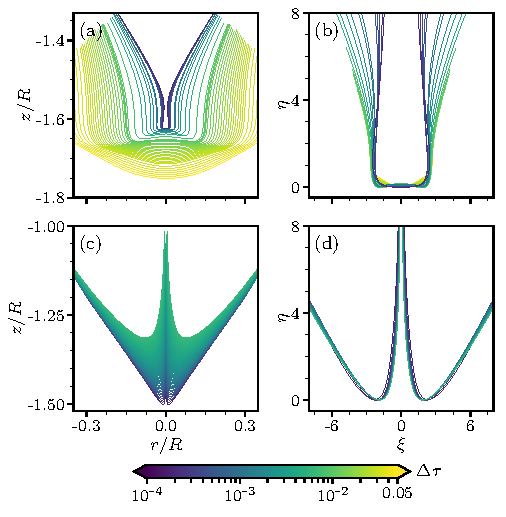
\includegraphics[width=\columnwidth]{fig3_Oh0.03_collapse.pdf}
\caption{Self-similar collapse of the interface for $Bo=0$ and $Oh=0.03$. Panels (a,c) show the raw shapes before and after jet inception. Panels (b,d) show the same profiles rescaled with $\xi=r/|\tau-\tau_0|^\alpha$ and $\eta=[z-z_j(\tau)]/|\tau-\tau_0|^\alpha$, using $\tau_0-\tau$ before inception, $\tau-\tau_0$ after inception, and $\alpha=0.629$. Colours indicate $\Delta\tau=|\tau-\tau_0|$. The post-inception jet collapse persists over more than two decades in dimensionless time; before inception the flanks collapse while the neck shrinks faster, following the equations governing the pinch-off of bubbles, as shown in \cite{PRF2023,PRL2024}.}
\label{fig:collapse}
\end{figure}
\emph{Conclusion.}---We have derived a family of self-similar solutions of the incompressible Euler equations for the collapse of a conical gas cavity of semiangle $\beta$. The jet radius and velocity scale as $r_j(\tau)\propto \tau^{1/(2-\nu(\beta))}$ and $v_j(\tau)\propto \tau^{(\nu(\beta)-1)/(2-\nu(\beta))}$, with $\nu(\beta)$ the degree of the Legendre function satisfying $P_\nu(-\cos\beta)=0$. For the measured bubble-entrapment range $35^\circ\lesssim\beta\lesssim41^\circ$, this gives $0.62\lesssim1/(2-\nu)\lesssim0.64$, close enough to $2/3$ to explain why inertio-capillary scalings appeared plausible.
The evidence for the balance comes directly from $We_j$, not only from the fitted exponent. In the self-similar region, $We_j(\tau)\propto \tau^{(2\nu-1)/(2-\nu)}$ diverges as $\tau\rightarrow0$, and the DNS gives both $We_j\gg1$ and a two-decade collapse of the free surface near the jet base when lengths are scaled with $r_j\propto\tau^{1/(2-\nu[\beta(Oh)])}$. Thus $Oh$ controls access to the singularity by selecting $\beta$, the inception time, and the regularisation scale; once the similarity window exists, the local collapse is governed by inertia.

Matching this inertial similarity to the viscous cutoff gives incipient radii $R_m\sim\mathcal{O}(1)$ nm for water bubbles with $R\sim15\,\mu$m, suggesting that bubble bursting can produce nanometric aerosol precursors to cloud condensation nuclei and ice-nucleating particles. The same $\beta$-sensitivity also gives a natural interpretation of shallow-layer simulations, where wall proximity steepens the focusing cavity and produces smaller jet drops \cite{YangShallow2026}; in the present convention, this corresponds to a smaller effective $\beta$, larger $v_M$, and smaller $R_m$. Testing the aerosol consequence now requires the physics outside the local similarity problem, including asymmetry, contaminants, particles, and gas-phase effects at the submicrometric scales of the thinnest jets \cite{MacIntyre,Bigg,PNAS,AnnRevDeike,PNASWang,Abyss,Eshima2026,JFM2026,PRLBird}.

\begin{acknowledgements}
This research work has been partially supported by the Grants PID2024-156545NB-I00 and PID2023-146809OB-I00, financed by the Spanish MICIU/AEI/10.13039/501100011033 and by ERDF/EU. V.S. acknowledges start-up funding from Durham University. This work made use of the Hamilton HPC Service of Durham University. The simulation work was also carried out on the national e-infrastructure of SURFsara, a subsidiary of SURF cooperation, the collaborative ICT organisation for Dutch education and research; this simulation work was sponsored by NWO~-- Domain Science for the use of supercomputer facilities.
\end{acknowledgements}


\nocite{Tian2023,wagner1932,AMZhang2026,Thoroddsen_18,Thoroddsen_2020}
\bibliography{Gordillo_bibv2}


\section*{\texorpdfstring{\NoCaseChange{End Matter}}{End Matter}}


\begin{figure*}[t]
\centering
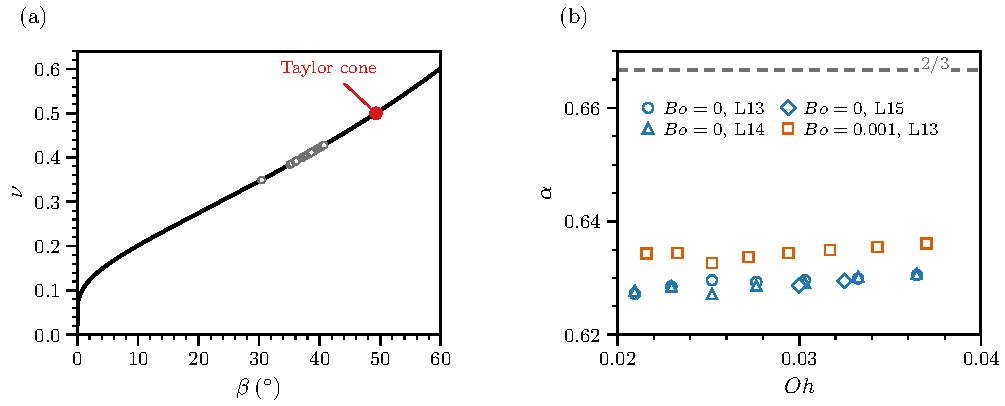
\includegraphics[width=0.925\textwidth]{nu_vs_beta.pdf}
\caption{(a) Values of $\nu$ solving Eq.~(\ref{condition}) as a function of the cone angle $\beta$; the grey symbols are the cone angles measured in the DNS. The red dot marks Taylor's cone, $\beta=49.3^\circ$, $\nu=0.5$. (b) Exponent $\alpha=1/(2-\nu)$ as a function of $Oh$ for $Bo=0$ (levels 13--15) and $Bo=10^{-3}$ (level 13), using the same cone fits; marker shapes distinguish refinement levels. The dashed line marks $\alpha=2/3$.
}
\label{fig:nu_vs_beta}
\end{figure*}

\subsection*{\texorpdfstring{\NoCaseChange{Numerical methods and data availability}}{Numerical methods and data availability}}

We solve the axisymmetric two--phase incompressible Navier--Stokes equations with the free software \textit{Basilisk C} \cite{Popinet2009,Popinet2015,Vatsal2021}. The interface is represented using a geometric volume-of-fluid field $c$, with density and viscosity interpolated in the one-fluid formulation. In dimensional form, the governing equations are
\begin{align}
\nabla\cdot\mathbf{u}
&\;= 0,
\label{eq:dns-incompressibility}\\
\rho(c)\left(\partial_t\mathbf{u}+\mathbf{u}\cdot\nabla\mathbf{u}\right)
&\;= -\nabla p+\nabla\cdot\left[2\mu(c)\mathbf{D}\right]+\sigma\kappa\delta_s\mathbf{n},
\label{eq:dns-momentum}
\end{align}
where $\mathbf{D}=\left[\nabla\mathbf{u}+(\nabla\mathbf{u})^T\right]/2$. Lengths, velocities, time, and pressure are scaled with $R$, $V_c=\sqrt{\sigma/(\rho_l R)}$, $R/V_c$, and $\sigma/R$, respectively. We fix $\rho_g/\rho_l=10^{-3}$ and $\mu_g/\mu_l=2\times10^{-2}$; all results reported in the Letter use $Bo=0$ and $Oh\simeq0.03$, unless stated otherwise.

For $Bo=0$, the initial condition is a spherical bubble of radius $R$ intersecting a flat free surface. The point contact is regularised by a capillary bridge of size $\delta=0.01R$, leaving an initial opening of radius $\simeq2\delta$. The computational domain spans $-6\le z/R\le4$ and $0\le r/R\le10$ for the production cases; the lower axial boundary is a no-slip, no-penetration wall, the upper axial boundary is an outflow, and $r=0$ is the axis of symmetry.

Adaptive mesh refinement is applied to the volume fraction, velocity, and curvature fields. To resolve the focusing singularity at jet inception, we developed a feature-tracking refinement criterion that follows the largest incoming curvature wave before inception and the newly formed jet thereafter. Data used in Figs.~\ref{fig:data-figs} and~\ref{fig:collapse} use $MAXlevel=15$, corresponding to a finest cell size $\Delta/R=10/2^{15}\simeq3.1\times10^{-4}$.

Grid independence is checked in Fig.~\ref{fig:data-figs} by repeating the $Oh\simeq0.03$ case at $MAXlevel=13$, 14, and 15. At $MAXlevel=15$, we also vary the focus level, defined here as the temporary pre-inception refinement cap used while tracking the focusing curvature wave before the mesh is released to $MAXlevel=15$ after jet inception. The results for focus levels 13--15 collapse onto the same scaling over the fitted asymptotic window.

The plotted scalings use the $MAXlevel=15$ data, resolve the jet base down to $r_j\simeq5\times10^{-3}$, and fit the asymptotic window $0.005\le r_j\le0.024$. The jet radius is the outer free-surface base returned by a tag-based probe that excludes detached droplets and entrained gas satellites; the base fluxes are integrated across the same axial plane (see Fig.~\ref{fig:data-figs}).

\noindent\textbf{Code availability.} The solver, case files, and post-processing scripts required to reproduce the figures in this Letter will be available at the public CoMPhy Lab repository \cite{BurstingBubbleCode}.

\subsection{\texorpdfstring{Solution to the equation $P_\nu(-\cos\beta) = 0$}{Solution to the equation Pnu(-cos beta) = 0}}

For each $\beta$, Eq.~(\ref{condition}) is solved as a scalar root-finding problem for the real degree $\nu$ of $P_\nu(-\cos\beta)$, choosing the branch continuous with Taylor's cone, $\beta=49.3^\circ$ and $\nu=1/2$. Fig.~\ref{fig:nu_vs_beta}(a) shows this mapping; panel (b) converts the DNS-measured cone angles into $\alpha=1/(2-\nu)$ as a function of $Oh$. The exponents are systematically below $2/3$ and vary with $Oh$, providing additional evidence against a fixed inertio-capillary exponent and in favour of the inertial conical-collapse similarity.

\end{document}

In the case in which the numerical simulations revealed that the streamlines are not perfectly perpendicular to the cone, the small tangential component of the velocity field at the interface would not contribute to the shrinking of the cavity and, hence, would not influence the jet ejection process, which could be also described by imposing $\phi=0$ at the interface.
